
\documentclass[10pt]{beamer}\usepackage[]{graphicx}\usepackage[]{xcolor}
% maxwidth is the original width if it is less than linewidth
% otherwise use linewidth (to make sure the graphics do not exceed the margin)
\makeatletter
\def\maxwidth{ %
  \ifdim\Gin@nat@width>\linewidth
    \linewidth
  \else
    \Gin@nat@width
  \fi
}
\makeatother

\definecolor{fgcolor}{rgb}{0.345, 0.345, 0.345}
\newcommand{\hlnum}[1]{\textcolor[rgb]{0.686,0.059,0.569}{#1}}%
\newcommand{\hlsng}[1]{\textcolor[rgb]{0.192,0.494,0.8}{#1}}%
\newcommand{\hlcom}[1]{\textcolor[rgb]{0.678,0.584,0.686}{\textit{#1}}}%
\newcommand{\hlopt}[1]{\textcolor[rgb]{0,0,0}{#1}}%
\newcommand{\hldef}[1]{\textcolor[rgb]{0.345,0.345,0.345}{#1}}%
\newcommand{\hlkwa}[1]{\textcolor[rgb]{0.161,0.373,0.58}{\textbf{#1}}}%
\newcommand{\hlkwb}[1]{\textcolor[rgb]{0.69,0.353,0.396}{#1}}%
\newcommand{\hlkwc}[1]{\textcolor[rgb]{0.333,0.667,0.333}{#1}}%
\newcommand{\hlkwd}[1]{\textcolor[rgb]{0.737,0.353,0.396}{\textbf{#1}}}%
\let\hlipl\hlkwb

\usepackage{framed}
\makeatletter
\newenvironment{kframe}{%
 \def\at@end@of@kframe{}%
 \ifinner\ifhmode%
  \def\at@end@of@kframe{\end{minipage}}%
  \begin{minipage}{\columnwidth}%
 \fi\fi%
 \def\FrameCommand##1{\hskip\@totalleftmargin \hskip-\fboxsep
 \colorbox{shadecolor}{##1}\hskip-\fboxsep
     % There is no \\@totalrightmargin, so:
     \hskip-\linewidth \hskip-\@totalleftmargin \hskip\columnwidth}%
 \MakeFramed {\advance\hsize-\width
   \@totalleftmargin\z@ \linewidth\hsize
   \@setminipage}}%
 {\par\unskip\endMakeFramed%
 \at@end@of@kframe}
\makeatother

\definecolor{shadecolor}{rgb}{.97, .97, .97}
\definecolor{messagecolor}{rgb}{0, 0, 0}
\definecolor{warningcolor}{rgb}{1, 0, 1}
\definecolor{errorcolor}{rgb}{1, 0, 0}
\newenvironment{knitrout}{}{} % an empty environment to be redefined in TeX

\usepackage{alltt}

\usepackage{xcolor}
\usepackage{mathtools}
\usepackage{graphicx} 
\usepackage{amsmath}
\usepackage{listings}
\lstnewenvironment{rc}[1][]{\lstset{language=R}}{}

\graphicspath{{images/}}
\usepackage{tikz} 
\usetikzlibrary{arrows,calc,patterns,positioning,shapes,decorations.markings} 
\usetikzlibrary{decorations.pathmorphing} 

%\usetheme{default}
\mode<presentation>
{
	\usetheme{Singapore}
	\usecolortheme{crane}
	% or ...
	
	\setbeamercovered{transparent}
	% or whatever (possibly just delete it)
}

%\title{Intro and regression}
%\subtitle{Introduction to Structural Equation Modeling using lavaan}
%Utrecht University Summer School: \\
%Introduction to Structural Equation Modeling using lavaan}
\title{Introduction to Structural Equation Modeling using lavaan}
\subtitle{Intro and regression}
\author{R. M. Kuiper (and many others)}
\institute{Department of Methodology \& Statistics \\ Utrecht University}
\date{}

%------------------------------------------------------------------------------%
\hypersetup{bookmarksdepth=-2}
\AtBeginSection[]
{
    \begin{frame}
        \frametitle{Table of Contents}
        \tableofcontents[currentsection]
    \end{frame}
}
\IfFileExists{upquote.sty}{\usepackage{upquote}}{}
\begin{document}


%------------------------------------------------------------------------------%

\begin{frame}[t, plain]
  \titlepage
\end{frame}

%------------------------------------------------------------------------------%
%
\begin{frame}{Outline of this lecture}
\tableofcontents
\end{frame}

%------------------------------------------------------------------------------%
%------------------------------------------------------------------------------%

\section{SEM}

%------------------------------------------------------------------------------%
%
% TO DO Lela mooi maken en mij vertellen hoe ik het aanpas?!
% En de twee arrows wat meer naar links?
\begin{frame}{Path Diagram: Graphical representation of SEM}

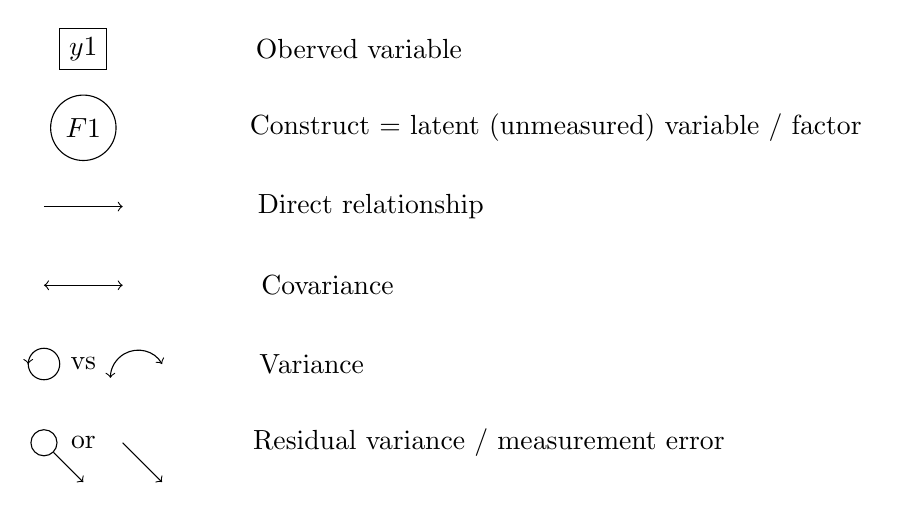
\begin{tikzpicture}
  \node[rectangle,draw=black] (y1) at (0,6) {$y1$}; 
  \node[draw=none,fill=none] at (3.5,6) {Oberved variable};
  %
  \node[circle,draw=black] (f1) at (0,5) {$F1$}; 
  \node[draw=none,fill=none] at (6,5) {Construct = latent (unmeasured) variable / factor};
  %
  \draw[->](-0.5,4) -- (0.5,4);
  \node[draw=none,fill=none] at (3.65,4) {Direct relationship};
  %
  \draw[<->](-0.5,3) -- (0.5,3);
  \node[draw=none,fill=none] at (3.1,3) {Covariance};
  %
  \draw[decoration={markings, mark=at position 0.5 with {\arrow{>}}},
        postaction={decorate}] (-0.5,2) circle (0.2);
  \node[draw=none,fill=none] at (0, 2) {vs};       
  \draw [<->] (1,2) arc (30:180:10pt);   
  \node[draw=none,fill=none] at (2.9,2) {Variance};   
  %
  \node[circle,draw=black] (c) at (-0.5,1){};
  \draw[->] (c) -- (0,0.5);
  \node[draw=none,fill=none] at (0, 1) {or}; 
  \draw[->](0.5,1) -- (1,0.5);
  \node[draw=none,fill=none] at (5.15,1) {Residual variance / measurement error}; 
\end{tikzpicture}


\end{frame}

%------------------------------------------------------------------------------%
  
\begin{frame}{Path models}

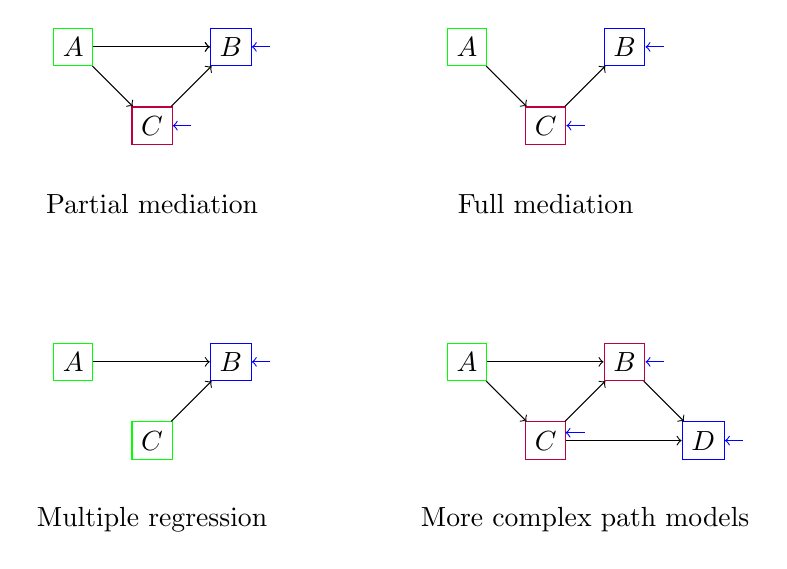
\begin{tikzpicture}

\node[rectangle,draw=green] (A2) at (0,5) {$A$}; 
\node[rectangle,draw=blue] (B2) at (2,5) {$B$}; 
\node[rectangle,draw=green] (C2) at (1,4) {$C$};
\node[draw=none,fill=none] at (1,3) {Multiple regression};
\draw[->] (A2) -- (B2);
\draw[->] (C2) -- (B2);
\draw[->, blue] (2.5,5) -- (B2);

\node[rectangle,draw=green] (A4) at (5,5) {$A$}; 
\node[rectangle,draw=purple] (B4) at (7,5) {$B$}; 
\node[rectangle,draw=purple] (C4) at (6,4) {$C$};
\node[rectangle,draw=blue] (D4) at (8,4) {$D$};
\node[draw=none,fill=none] at (6.5,3) {More complex path models};
\draw[->] (A4) -- (B4);
\draw[->] (A4) -- (C4);
\draw[->] (C4) -- (B4);
\draw[->] (C4) -- (D4);
\draw[->] (B4) -- (D4);
\draw[->, blue] (7.5,5) -- (B4);
\draw[->, blue] (6.5,4.1) -- (6.25,4.1);
\draw[->, blue] (8.5,4) -- (D4);

\node[rectangle,draw=green] (A1) at (0,9) {$A$}; 
\node[rectangle,draw=blue] (B1) at (2,9) {$B$};
\node[rectangle,draw=purple](C1) at (1,8) {$C$};
\node[draw=none,fill=none] at (1,7) {Partial mediation};
\draw[->] (A1) -- (B1);
\draw[->] (A1) -- (C1);
\draw[->] (C1) -- (B1);
\draw[->] (A1) -- (B1);
\draw[->, blue] (2.5,9) -- (B1);
\draw[->, blue] (1.5,8) -- (C1);

\node[rectangle,draw=green] (A3) at (5,9) {$A$}; 
\node[rectangle,draw=blue] (B3) at (7,9) {$B$};
\node[rectangle,draw=purple] (C3) at  (6,8) {$C$}; 

\node[draw=none,fill=none] at (6,7) {Full mediation};
\draw[->] (A3) -- (C3);
\draw[->] (C3) -- (B3);
\draw[->, blue] (7.5,9) -- (B3);
\draw[->, blue] (6.5,8) -- (C3);

\end{tikzpicture}

\end{frame}
%------------------------------------------------------------------------------%
  
\begin{frame}{Measurement models}
\begingroup
\centering

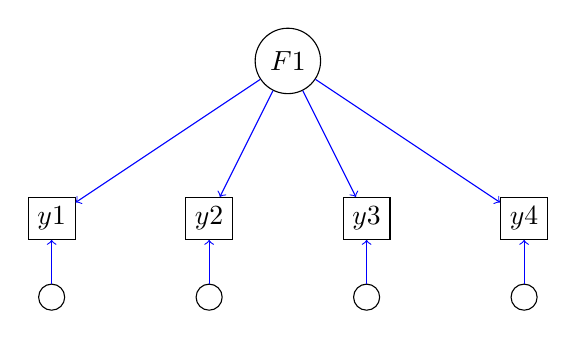
\begin{tikzpicture}
\node[circle,draw=black] (f1) at (4,4) {$F1$}; 
\node[rectangle,draw=black] (y1) at (1,2) {$y1$};
\node[rectangle,draw=black] (y2) at (3,2) {$y2$}; 
\node[rectangle,draw=black] (y3) at (5,2) {$y3$}; 
\node[rectangle,draw=black] (y4) at (7,2) {$y4$}; 
\node[circle,draw=black] (u1) at (1,1){};
\node[circle,draw=black] (u2) at (3,1){};
\node[circle,draw=black] (u3) at (5,1){};
\node[circle,draw=black] (u4) at (7,1){};
\draw[->, blue] (f1) -- (y1);
\draw[->, blue] (f1) -- (y2);
\draw[->, blue] (f1) -- (y3);
\draw[->, blue] (f1) -- (y4);
\draw[->, blue] (u1) -- (y1);
\draw[->, blue] (u2) -- (y2);
\draw[->, blue] (u3) -- (y3);
\draw[->, blue] (u4) -- (y4);
\end{tikzpicture}

\endgroup
\end{frame}     
%------------------------------------------------------------------------------%
\begin{frame}{SEM}
\begin{itemize}
    \item From theory to model (and path diagram)
    \item Compare
\end{itemize}

\includegraphics[height=5cm,keepaspectratio=T] {SEM_example.png}
\end{frame}
%------------------------------------------------------------------------------%
%
%------------------------------------------------------------------------------%
\section{SAPI}
%------------------------------------------------------------------------------%
%
%------------------------------------------------------------------------------%
%
\begin{frame}{Example: South African Personality Inventory Project (SAPI)}

\includegraphics[height=7.5cm,keepaspectratio=T] {SAPI.png}

\end{frame}
%------------------------------------------------------------------------------%
%
\begin{frame}{SAPI details for this lecture}

Our data: 
\begin{itemize}
    \item Selection of 1000 participants.
    \item Selection of 7 out of 262 personality items:
        \begin{itemize}
        \item Regression:
          \begin{itemize}
          \item{Outcome: Q77, I enjoy telling funny stories}
          \item{Predictor: Age}
          \end{itemize}
        \item Path model:
          \begin{itemize}
          \item{Outcome: Q196, I make others laugh}
          \item{Mediator: Q77, \ I enjoy telling funny stories}
          \item{Predictor: Age}
          \end{itemize}
        \item Later, we use: Age, ReadAb, Q44, Q63, and Q76.
        \end{itemize}
\end{itemize}
\end{frame}
%------------------------------------------------------------------------------%
%
%------------------------------------------------------------------------------%
\section{Lavaan commands}
%------------------------------------------------------------------------------%
%
%------------------------------------------------------------------------------%
%
\begin{frame}{Steps to take for running a model in lavaan}

\begin{itemize}
\item{1. Loading data into R}
\item{2. Data screening: \\
e.g., check measurement levels, missing data (notation),
and correlations.}
\item{3. Draw your model}
\item{4. Specify your model in lavaan}
\item{5. Fit the model with lavaan}
\item{6. Plot the lavaan model in R}
\item{7. Ensure model specification is correct
using plots and technical output.\\
If not, correct and proceed from Step 4 on.}
\item{8. Check model assumptions: \\
e.g., check residuals (histogram or Q-Q plot).}
\item{9. Acquire the summary from lavaan}
\item{And more steps, discussed later on.}
\end{itemize}

\end{frame}
%------------------------------------------------------------------------------%
\begin{frame}[fragile]{1. Loading data into R}

For example, in case of a .txt file:

\begin{knitrout}
\definecolor{shadecolor}{rgb}{0.969, 0.969, 0.969}\color{fgcolor}\begin{kframe}
\begin{alltt}
\hldef{data_sapi} \hlkwb{<-} \hlkwd{read.table}\hldef{(}\hlsng{"Sapi.txt"}\hldef{,} \hlkwc{header} \hldef{= T)}

\hldef{data_sapi[}\hlkwd{sapply}\hldef{(data_sapi,}
    \hlkwa{function}\hldef{(}\hlkwc{x}\hldef{)} \hlkwd{as.character}\hldef{(x)} \hlopt \hlkwd{c}\hldef{(}\hlsng{"-999"}\hldef{) )]} \hlkwb{<-} \hlnum{NA}
\end{alltt}
\end{kframe}
\end{knitrout}

\end{frame}
%------------------------------------------------------------------------------%
%
\begin{frame}[fragile]{3. Draw your model}

\includegraphics[height=2cm, keepaspectratio=T] {RegressionModel.png}

\end{frame}
%------------------------------------------------------------------------------%
%
\begin{frame}[fragile]{4. Specify your model}

\includegraphics[height=2cm, keepaspectratio=T] {RegressionModel.png}

\begin{itemize}
  \item Translate $\,\to\,$ into $\sim$.
  \item Translate 'residual variance notation' into $\sim\sim$.\\
  Note = residual variance = a variance = special case covariance.
  \item Translate $\xleftrightarrow{}$ (= covariance) into $\sim\sim$.
  \item Do not forget about intercepts: Translate into $\sim$.
  
  \vspace{5mm}
  
  \item Translate 'circled arrow' (= variance) into $\sim\sim$.\\
  Note = variance = special case covariance.
  \item Do not forget about means: Translate into $\sim$.
\end{itemize}
    
\end{frame}
%------------------------------------------------------------------------------%
%
\begin{frame}[fragile]{4. Specify your model: regression SAPI}

\includegraphics[height=2cm, keepaspectratio=T] {RegressionModel.png}

\begin{itemize}
  \item Translate $\,\to\,$ into $\sim$.
  \item Translate 'residual variance notation' into $\sim\sim$.\\
  Note = residual variance = a variance = special case covariance.
  \item Translate $\xleftrightarrow{}$ (= covariance) into $\sim\sim$.
  \item Do not forget about intercepts: Translate into $\sim$.
\end{itemize}

\begin{knitrout}
\definecolor{shadecolor}{rgb}{0.969, 0.969, 0.969}\color{fgcolor}\begin{kframe}
\begin{alltt}
\hldef{mod.regr} \hlkwb{<-} \hlsng{'
  Q77 ~ Age  # regression
  Q77 ~~ Q77 # residual variance
  Q77 ~ 1    # intercept
'}
\end{alltt}
\end{kframe}
\end{knitrout}

\end{frame}
%------------------------------------------------------------------------------%
%
\begin{frame}[fragile]{4. Specify your model: regression general}

A regression model is specified as follows: \\
dependent $\sim$ predictor1 + predictor2 + etc.\\

\vspace{5mm}

Additionally, one needs to specify that the error (of the dependent variable) has a variance:\\
dependent $\sim$$\sim$ dependent\\ 

\vspace{5mm}

If needed, one can specify to include an intercept:\\
dependent $\sim$ 1\\

\vspace{5mm}

Note that one include intercept directly: \\
dependent $\sim$ 1 + predictor1 + predictor2 + etc.


\end{frame}
%------------------------------------------------------------------------------%
%
\begin{frame}[fragile]{4. Specify your model: regression DIY}

\includegraphics[height=6cm, keepaspectratio=T] {regression_DIY.png}

\begin{itemize}
  \item Do you recognize this model? 
  \item Specify this in lavaan code. \\
  Do not forget the parameters that are not drawn, but do are there.
\end{itemize}

\end{frame}
%------------------------------------------------------------------------------%
%
\begin{frame}[fragile]{4. Specify your model: regression answer}

\includegraphics[height=2cm, keepaspectratio=T] {regression_DIY.png} 

\begin{knitrout}
\definecolor{shadecolor}{rgb}{0.969, 0.969, 0.969}\color{fgcolor}\begin{kframe}
\begin{alltt}
\hldef{mod.regr_DIY} \hlkwb{<-} \hlsng{'
  y2 ~ 1 + x1 + x2  # intercept + regression
  y2 ~~ y2          # residual variance
  
  # Make it a habit to also specify:
  x1 ~ 1            # mean x1 
  x2 ~ 1            # mean x2 
  x1 ~~ x1          # variance x1 
  x1 ~~ x2          # covariance x1 and x2
  x2 ~~ x2          # variance x2
'}
\end{alltt}
\end{kframe}
\end{knitrout}

\end{frame}
%------------------------------------------------------------------------------%
%
\begin{frame}[fragile]{4. Specify your model: regression answer 2}

\includegraphics[height=2cm, keepaspectratio=T] {regression_DIY.png} 

\begin{knitrout}
\definecolor{shadecolor}{rgb}{0.969, 0.969, 0.969}\color{fgcolor}\begin{kframe}
\begin{alltt}
\hldef{mod.regr_DIY} \hlkwb{<-} \hlsng{'
  y2 ~ 1 + x1 + x2  # intercept + regression
  y2 ~~ y2          # residual variance
  
  # Make it a habit to also specify:
  x1 + x2 ~ 1       # means predictors - DO specify this!
  x1 + x2 ~~ x1     # (co)variance predictors 
  x2 ~~ x2          # variance x2
'}
\end{alltt}
\end{kframe}
\end{knitrout}

\textcolor{red}{Note:} As opposed to what I say in the video, do specify the means for the predictors explicitly; otherwise they will be set to 0.

\end{frame}
%------------------------------------------------------------------------------%
%
\begin{frame}[fragile]{4. Specify your model: regression answer general}

\begin{verbatim}
  y ~ 1 + x_1 + x_2 + ... + x_k  # intercept + regression
  y ~~ y                         # residual variance
  
  # (co)variances of exogenous variables:
  x_1 + x_2 + ... + x_k ~~ x_1
        x_2 + ... + x_k ~~ x_2
                        ...
                    x_k ~~ x_k
\end{verbatim}

\end{frame}
%------------------------------------------------------------------------------%
%
\subsection*{Lavaan commands - Part 2}
%------------------------------------------------------------------------------%
%
\begin{frame}[fragile]{5. Fit the regression model}

\begin{knitrout}
\definecolor{shadecolor}{rgb}{0.969, 0.969, 0.969}\color{fgcolor}\begin{kframe}
\begin{alltt}
\hldef{fit.regr} \hlkwb{<-} \hlkwd{lavaan}\hldef{(}\hlkwc{model} \hldef{= mod.regr,} \hlkwc{data} \hldef{= data_sapi)}
\end{alltt}
\end{kframe}
\end{knitrout}
\end{frame}
%------------------------------------------------------------------------------%
%
\begin{frame}[fragile]{5. Fit the regression model: All code}

\begin{knitrout}
\definecolor{shadecolor}{rgb}{0.969, 0.969, 0.969}\color{fgcolor}\begin{kframe}
\begin{alltt}
\hlcom{# Data}
\hldef{data_sapi} \hlkwb{<-} \hlkwd{read.table}\hldef{(}\hlsng{"Sapi.txt"}\hldef{,} \hlkwc{header} \hldef{= T)}
\hldef{data_sapi[}\hlkwd{sapply}\hldef{(data_sapi,}
    \hlkwa{function}\hldef{(}\hlkwc{x}\hldef{)} \hlkwd{as.character}\hldef{(x)} \hlopt \hlkwd{c}\hldef{(}\hlsng{"-999"}\hldef{) )]} \hlkwb{<-} \hlnum{NA}

\hlcom{# Model}
\hldef{mod.regr} \hlkwb{<-} \hlsng{'
  Q77 ~ Age  # regression
  Q77 ~~ Q77 # residual variance
  Q77 ~ 1    # intercept
'}

\hlcom{# Fit model}
\hldef{fit.regr} \hlkwb{<-} \hlkwd{lavaan}\hldef{(}\hlkwc{model} \hldef{= mod.regr,} \hlkwc{data} \hldef{= data_sapi)}
\end{alltt}
\end{kframe}
\end{knitrout}
\end{frame}
%------------------------------------------------------------------------------%
%
\begin{frame}{6. Plot the lavaan model in R}
\begin{itemize}
  \item{lavaanPlot}
  \item{graph\_sem from tidySEM} 
  \item{semPaths from semPlot}
  \item{probably many more...}
\end{itemize}

\end{frame}
%------------------------------------------------------------------------------%
%
\begin{frame}[fragile]{Plot with lavaanPlot}
\small{
\begin{knitrout}
\definecolor{shadecolor}{rgb}{0.969, 0.969, 0.969}\color{fgcolor}\begin{kframe}
\begin{alltt}
\hlkwa{if} \hldef{(}\hlopt{!}\hlkwd{require}\hldef{(}\hlsng{"lavaanPlot"}\hldef{))} \hlkwd{install.packages}\hldef{(}\hlsng{"lavaanPlot"}\hldef{)}
\hlkwd{library}\hldef{(lavaanPlot)}
\end{alltt}
\end{kframe}
\end{knitrout}
\begin{knitrout}
\definecolor{shadecolor}{rgb}{0.969, 0.969, 0.969}\color{fgcolor}\begin{kframe}
\begin{alltt}
\hlkwd{lavaanPlot}\hldef{(}\hlkwc{model} \hldef{= fit.regr,}
           \hlkwc{graph_options} \hldef{=} \hlkwd{list}\hldef{(}\hlkwc{overlap} \hldef{=} \hlsng{"true"}\hldef{,}
                                \hlkwc{fontsize} \hldef{=} \hlsng{"20"}\hldef{),}
           \hlkwc{node_options} \hldef{=} \hlkwd{list}\hldef{(}\hlkwc{shape} \hldef{=} \hlsng{"box"}\hldef{,}
                               \hlkwc{fontname} \hldef{=} \hlsng{"Helvetica"}\hldef{),}
           \hlkwc{edge_options} \hldef{=} \hlkwd{list}\hldef{(}\hlkwc{color} \hldef{=} \hlsng{"grey"}\hldef{),}
           \hlkwc{coefs} \hldef{= T,} \hlkwc{stand} \hldef{= T,} \hlkwc{covs} \hldef{= T,}
           \hldef{)}
\end{alltt}
\end{kframe}
\end{knitrout}
}
\end{frame}
%------------------------------------------------------------------------------%
%
\begin{frame}[fragile]{Plot with tidySEM}
\begin{knitrout}
\definecolor{shadecolor}{rgb}{0.969, 0.969, 0.969}\color{fgcolor}\begin{kframe}
\begin{alltt}
\hlkwd{library}\hldef{(tidySEM)}
\hlkwa{if} \hldef{(}\hlopt{!}\hlkwd{require}\hldef{(}\hlsng{"tidySEM"}\hldef{))} \hlkwd{install.packages}\hldef{(}\hlsng{"tidySEM"}\hldef{)}
\end{alltt}
\end{kframe}
\end{knitrout}
\begin{knitrout}
\definecolor{shadecolor}{rgb}{0.969, 0.969, 0.969}\color{fgcolor}\begin{kframe}
\begin{alltt}
\hlkwd{graph_sem}\hldef{(fit.regr)}
\end{alltt}
\end{kframe}
\end{knitrout}
\end{frame}
%------------------------------------------------------------------------------%
%
\begin{frame}[fragile]{Plot with semPlot}

\begin{knitrout}
\definecolor{shadecolor}{rgb}{0.969, 0.969, 0.969}\color{fgcolor}\begin{kframe}
\begin{alltt}
\hlkwa{if} \hldef{(}\hlopt{!}\hlkwd{require}\hldef{(}\hlsng{"semPlot"}\hldef{))} \hlkwd{install.packages}\hldef{(}\hlsng{"semPlot"}\hldef{)}
\hlkwd{library}\hldef{(semPlot)}
\end{alltt}
\end{kframe}
\end{knitrout}
\begin{knitrout}
\definecolor{shadecolor}{rgb}{0.969, 0.969, 0.969}\color{fgcolor}\begin{kframe}
\begin{alltt}
\hlkwd{semPaths}\hldef{(fit.regr,} \hlsng{"par"}\hldef{,} \hlkwc{weighted} \hldef{=} \hlnum{FALSE}\hldef{,} \hlkwc{nCharNodes} \hldef{=} \hlnum{7}\hldef{,}
         \hlkwc{shapeMan} \hldef{=} \hlsng{"rectangle"}\hldef{,} \hlkwc{sizeMan} \hldef{=} \hlnum{8}\hldef{,} \hlkwc{sizeMan2} \hldef{=} \hlnum{5}\hldef{)}
\end{alltt}
\end{kframe}
\end{knitrout}
\end{frame}
%------------------------------------------------------------------------------%
%
\begin{frame}[fragile]{9. Acquiring the summary}

\begin{knitrout}
\definecolor{shadecolor}{rgb}{0.969, 0.969, 0.969}\color{fgcolor}\begin{kframe}
\begin{alltt}
\hlkwd{summary}\hldef{(fit.regr,} \hlkwc{fit.measures} \hldef{=} \hlnum{TRUE}\hldef{,}
        \hlkwc{ci} \hldef{=} \hlnum{TRUE}\hldef{,} \hlkwc{rsquare} \hldef{=} \hlnum{TRUE}\hldef{)}
\end{alltt}
\end{kframe}
\end{knitrout}

\begin{knitrout}
\definecolor{shadecolor}{rgb}{0.969, 0.969, 0.969}\color{fgcolor}\begin{kframe}
\begin{alltt}
\hlkwd{parameterEstimates}\hldef{(fit.regr)}

\hlkwd{inspect}\hldef{(fit.regr,} \hlsng{'r2'}\hldef{)}
\hlcom{# As an example, there are more.}

\hlkwd{fitMeasures}\hldef{(fit.regr,}
            \hlkwd{c}\hldef{(}\hlsng{"npar"}\hldef{,} \hlsng{"logl"}\hldef{,} \hlsng{"unrestricted.logl"}\hldef{,}
              \hlsng{"chisq"}\hldef{,} \hlsng{"pvalue"}\hldef{,}
              \hlsng{"cfi"}\hldef{,} \hlsng{"tli"}\hldef{,} \hlsng{"rmsea"}\hldef{))}
\hlcom{# As an example, there are more.}
\end{alltt}
\end{kframe}
\end{knitrout}

\end{frame}
%------------------------------------------------------------------------------%
%
%------------------------------------------------------------------------------%
\section{Regression}
%------------------------------------------------------------------------------%

\begin{frame}[fragile]{Analyzing the SAPI data: Regression}

Variables:
\begin{itemize}
\item{Outcome: Q77, I enjoy telling funny stories}
\item{Predictor: Age}
\end{itemize}

\vspace{5mm}

\includegraphics[height=2cm,keepaspectratio=T] {RegressionModel.png}

\end{frame}
%------------------------------------------------------------------------------%
%
\begin{frame}[fragile]{Specifying and fitting regression model in lavaan}
\begin{knitrout}
\definecolor{shadecolor}{rgb}{0.969, 0.969, 0.969}\color{fgcolor}\begin{kframe}
\begin{alltt}
\hldef{mod.regr} \hlkwb{<-} \hlsng{'
  Q77 ~  Age # regression
  Q77 ~~ Q77 # residual variance
  Q77 ~  1   # intercept
'}
\end{alltt}
\end{kframe}
\end{knitrout}

\vspace{5mm}

\begin{knitrout}
\definecolor{shadecolor}{rgb}{0.969, 0.969, 0.969}\color{fgcolor}\begin{kframe}
\begin{alltt}
\hldef{fit.regr} \hlkwb{<-} \hlkwd{lavaan}\hldef{(}\hlkwc{model} \hldef{= mod.regr,} \hlkwc{data} \hldef{= data_sapi)}
\end{alltt}
\end{kframe}
\end{knitrout}
\end{frame}
%------------------------------------------------------------------------------%
%
\begin{frame}[fragile]{Plot with lavaanPlot}
\small{
\begin{knitrout}
\definecolor{shadecolor}{rgb}{0.969, 0.969, 0.969}\color{fgcolor}\begin{kframe}
\begin{alltt}
  \hlkwd{lavaanPlot}\hldef{(}\hlkwc{model} \hldef{= fit.regr,}
           \hlkwc{graph_options} \hldef{=} \hlkwd{list}\hldef{(}\hlkwc{overlap} \hldef{=} \hlsng{"true"}\hldef{,}
                                \hlkwc{fontsize} \hldef{=} \hlsng{"20"}\hldef{),}
           \hlkwc{node_options} \hldef{=} \hlkwd{list}\hldef{(}\hlkwc{shape} \hldef{=} \hlsng{"box"}\hldef{,}
                               \hlkwc{fontname} \hldef{=} \hlsng{"Helvetica"}\hldef{),}
           \hlkwc{edge_options} \hldef{=} \hlkwd{list}\hldef{(}\hlkwc{color} \hldef{=} \hlsng{"grey"}\hldef{),}
           \hlkwc{coefs} \hldef{= T,} \hlkwc{stand} \hldef{= F,} \hlkwc{covs} \hldef{= T,}
           \hldef{)}
\end{alltt}
\end{kframe}
\includegraphics[width=4in]{figure/unnamed-chunk-17-1} 
\begin{kframe}\begin{alltt}
\hlcom{# Note: I use stand = F here.}
\end{alltt}
\end{kframe}
\end{knitrout}
}
\end{frame}
%------------------------------------------------------------------------------%
%
\begin{frame}[fragile]{Summary regression model in lavaan}

\begin{knitrout}
\definecolor{shadecolor}{rgb}{0.969, 0.969, 0.969}\color{fgcolor}\begin{kframe}
\begin{alltt}
\hlkwd{summary}\hldef{(fit.regr,} \hlkwc{fit.measures} \hldef{=} \hlnum{TRUE}\hldef{,}
        \hlkwc{ci} \hldef{=} \hlnum{TRUE}\hldef{,} \hlkwc{rsquare} \hldef{=} \hlnum{TRUE}\hldef{)}
\end{alltt}
\end{kframe}
\end{knitrout}

\vspace{5mm}

Estimates: 
\begin{knitrout}
\definecolor{shadecolor}{rgb}{0.969, 0.969, 0.969}\color{fgcolor}\begin{kframe}
\begin{alltt}
\hlkwd{parameterEstimates}\hldef{(fit.regr)[}\hlkwd{c}\hldef{(}\hlnum{1}\hldef{,}\hlnum{2}\hldef{,}\hlnum{3}\hldef{),]} \hlcom{# or ...[1:3,]}
\end{alltt}
\begin{verbatim}
##   lhs op rhs    est    se      z pvalue ci.lower ci.upper
## 1 Q77  ~ Age -0.022 0.004 -5.275      0   -0.030   -0.014
## 2 Q77 ~~ Q77  1.184 0.068 17.536      0    1.052    1.317
## 3 Q77 ~1      4.275 0.135 31.657      0    4.011    4.540
\end{verbatim}
\end{kframe}
\end{knitrout}
\end{frame}
%------------------------------------------------------------------------------%
%
\begin{frame}[fragile]{Regression equation}

\begin{knitrout}
\definecolor{shadecolor}{rgb}{0.969, 0.969, 0.969}\color{fgcolor}\begin{kframe}
\begin{alltt}
\hlkwd{parameterEstimates}\hldef{(fit.regr)[}\hlkwd{c}\hldef{(}\hlnum{1}\hldef{,}\hlnum{2}\hldef{,}\hlnum{3}\hldef{),]} \hlcom{# or ...[1:3,]}
\end{alltt}
\begin{verbatim}
##   lhs op rhs    est    se      z pvalue ci.lower ci.upper
## 1 Q77  ~ Age -0.022 0.004 -5.275      0   -0.030   -0.014
## 2 Q77 ~~ Q77  1.184 0.068 17.536      0    1.052    1.317
## 3 Q77 ~1      4.275 0.135 31.657      0    4.011    4.540
\end{verbatim}
\end{kframe}
\end{knitrout}

General regression equation (for person $i$):\\
$Q77_i = B_0 + B_1*Age_i + e_i$, with $e_i \sim N(0, \sigma^2)$.\\
Or: $\hat{Q77}_i = B_0 + B_1*Age_i$.

\vspace{5mm}

Regression equation (for person $i$):\\
$Q77_i = 4.275 - 0.022*Age_i + e_i$, with $e \sim N(0, 1.184)$.

\end{frame}
%------------------------------------------------------------------------------%
%
\begin{frame}
\includegraphics[height=6cm,keepaspectratio=T] {regression.png}
\end{frame}
%------------------------------------------------------------------------------%
%
\begin{frame}[fragile]{Summary regression model in lavaan Ctd.}
$R^2$ = R-squared = proportion of shared/explained variance:
\begin{knitrout}
\definecolor{shadecolor}{rgb}{0.969, 0.969, 0.969}\color{fgcolor}\begin{kframe}
\begin{alltt}
\hlkwd{inspect}\hldef{(fit.regr,} \hlsng{'r2'}\hldef{)}
\end{alltt}
\begin{verbatim}
##   Q77 
## 0.043
\end{verbatim}
\end{kframe}
\end{knitrout}
\end{frame}
%------------------------------------------------------------------------------%
%
\begin{frame}[fragile]{Intermezzo: Correlation Age and Q77 and $R^2$ in R}
\begin{knitrout}
\definecolor{shadecolor}{rgb}{0.969, 0.969, 0.969}\color{fgcolor}\begin{kframe}
\begin{alltt}
\hldef{corr} \hlkwb{<-} \hlkwd{cor}\hldef{(data_sapi[,} \hlnum{2}\hldef{], data_sapi[,} \hlnum{9}\hldef{],}
          \hlkwc{use} \hldef{=} \hlsng{"complete.obs"}\hldef{)}

\hlkwd{round}\hldef{(corr,} \hlnum{3}\hldef{)}   \hlcom{# = correlation between Age and Q77}
\end{alltt}
\begin{verbatim}
## [1] -0.208
\end{verbatim}
\end{kframe}
\end{knitrout}

\begin{knitrout}
\definecolor{shadecolor}{rgb}{0.969, 0.969, 0.969}\color{fgcolor}\begin{kframe}
\begin{alltt}
\hlkwd{round}\hldef{(corr}\hlopt{^}\hlnum{2}\hldef{,} \hlnum{3}\hldef{)} \hlcom{# = R^2}
\end{alltt}
\begin{verbatim}
## [1] 0.043
\end{verbatim}
\begin{alltt}
\hlcom{# R^2 = proportion of shared/explained variance. }
\hlcom{# This is the R^2 in a regression with one predictor.}
\end{alltt}
\end{kframe}
\end{knitrout}
In a regression with one outcome and one predictor,\\
the $R^2$ is the square of their correlation.
\end{frame}
%------------------------------------------------------------------------------%
%
\begin{frame}[fragile]{Intermezzo: Correlation Age and Q77 and $R^2$ in R Ctd.}

Remark:\\
I would not use lavaan for correlations, but you can:
\begin{knitrout}
\definecolor{shadecolor}{rgb}{0.969, 0.969, 0.969}\color{fgcolor}\begin{kframe}
\begin{alltt}
\hldef{mod.corr} \hlkwb{<-} \hlsng{'
  Q77 ~~ Q77
  Age ~~ Age
  Q77 ~~ Age # covariance
  # If standardized, then correlation
'}
\hldef{fit.corr} \hlkwb{<-} \hlkwd{lavaan}\hldef{(}\hlkwc{model} \hldef{= mod.corr,} \hlkwc{data} \hldef{= data_sapi)}
\hlkwd{parameterEstimates}\hldef{(fit.corr,} \hlkwc{stand}\hldef{=T)[}\hlnum{3}\hldef{,}\hlsng{'std.all'}\hldef{]}
\end{alltt}
\begin{verbatim}
## [1] -0.2080665
\end{verbatim}
\end{kframe}
\end{knitrout}

Message intermezzo:\\
In a regression with one outcome and one predictor,\\
the $R^2$ is the square of their correlation.
\end{frame}
%------------------------------------------------------------------------------%
%
%------------------------------------------------------------------------------%
\section{Path model}
%------------------------------------------------------------------------------%
%
\begin{frame}{Analyzing the SAPI data: Path model (Mediation)}

Variables:
\begin{itemize}
\item{Outcome: Q196, I make others laugh}
\item{Mediator: Q77, I enjoy telling funny stories}
\item{Predictor: Age}
\end{itemize}

\vspace{5mm}

\includegraphics[height=2cm,keepaspectratio=T] {path_model.png}

\end{frame}
%------------------------------------------------------------------------------%
%
\begin{frame}[fragile]{Specification path model in lavaan}

\begin{knitrout}
\definecolor{shadecolor}{rgb}{0.969, 0.969, 0.969}\color{fgcolor}\begin{kframe}
\begin{alltt}
\hldef{model.path} \hlkwb{<-} \hlsng{'
  # regressions
  Q77  ~ Age 
  Q196 ~ Q77 
  
  # residual variances
  Q77  ~~ Q77
  Q196 ~~ Q196
  
  # variance of predictor
  Age ~~ Age
  # mean of predictor
  Age ~ 1
  
  ## intercepts 
  Q77  ~ 1
  Q196 ~ 1
'}
\hldef{fit_path} \hlkwb{<-} \hlkwd{lavaan}\hldef{(}\hlkwc{model} \hldef{= model.path,} \hlkwc{data} \hldef{= data_sapi)}
\end{alltt}
\end{kframe}
\end{knitrout}

\end{frame}
%------------------------------------------------------------------------------%
%
\begin{frame}[fragile]{Plot with lavaanPlot}
\begin{knitrout}
\definecolor{shadecolor}{rgb}{0.969, 0.969, 0.969}\color{fgcolor}\begin{kframe}
\begin{alltt}
  \hlkwd{lavaanPlot}\hldef{(}\hlkwc{model} \hldef{= fit_path,}
           \hlkwc{graph_options} \hldef{=} \hlkwd{list}\hldef{(}\hlkwc{overlap} \hldef{=} \hlsng{"true"}\hldef{,}
                                \hlkwc{fontsize} \hldef{=} \hlsng{"20"}\hldef{),}
           \hlkwc{node_options} \hldef{=} \hlkwd{list}\hldef{(}\hlkwc{shape} \hldef{=} \hlsng{"box"}\hldef{,}
                               \hlkwc{fontname} \hldef{=} \hlsng{"Helvetica"}\hldef{),}
           \hlkwc{edge_options} \hldef{=} \hlkwd{list}\hldef{(}\hlkwc{color} \hldef{=} \hlsng{"grey"}\hldef{),}
           \hlkwc{coefs} \hldef{= T,} \hlkwc{stand} \hldef{= F,} \hlkwc{covs} \hldef{= T,}
           \hldef{)} \hlcom{# Note: stand = F}
\end{alltt}
\end{kframe}
\includegraphics[width=4in]{figure/unnamed-chunk-26-1} 
\end{knitrout}
\end{frame}
%------------------------------------------------------------------------------%
%
\begin{frame}[fragile]{Summary path model in lavaan}

\begin{knitrout}
\definecolor{shadecolor}{rgb}{0.969, 0.969, 0.969}\color{fgcolor}\begin{kframe}
\begin{alltt}
\hlkwd{summary}\hldef{(fit_path,} \hlkwc{fit.measures} \hldef{=} \hlnum{TRUE}\hldef{,}
        \hlkwc{ci} \hldef{=} \hlnum{TRUE}\hldef{,} \hlkwc{rsquare} \hldef{=} \hlnum{TRUE}\hldef{)}
\end{alltt}
\end{kframe}
\end{knitrout}

Estimates 
\begin{knitrout}
\definecolor{shadecolor}{rgb}{0.969, 0.969, 0.969}\color{fgcolor}\begin{kframe}
\begin{alltt}
\hlkwd{parameterEstimates}\hldef{(fit_path)[,}\hlopt{-}\hlnum{7}\hldef{]} \hlcom{# i.e., without p-value}
\end{alltt}
\begin{verbatim}
##    lhs op  rhs     est    se      z ci.lower ci.upper
## 1  Q77  ~  Age  -0.021 0.004 -4.971   -0.029   -0.013
## 2 Q196  ~  Q77   0.451 0.027 16.724    0.398    0.504
## 3  Q77 ~~  Q77   1.179 0.067 17.479    1.047    1.312
## 4 Q196 ~~ Q196   0.545 0.031 17.479    0.484    0.606
## 5  Age ~~  Age 108.692 6.219 17.479   96.504  120.881
## 6  Age ~1       30.612 0.422 72.580   29.785   31.439
## 7  Q77 ~1        4.248 0.136 31.175    3.981    4.516
## 8 Q196 ~1        2.153 0.102 21.167    1.954    2.352
\end{verbatim}
\end{kframe}
\end{knitrout}

%> mean(data_sapi[, 2], na.rm=T)
%[1] 30.7233
%> max(data_sapi[, 2], na.rm=T)
%[1] 73
%> min(data_sapi[, 2], na.rm=T)
%[1] 12
%> sd(data_sapi[, 2], na.rm=T)
%[1] 10.53663
\end{frame}
%------------------------------------------------------------------------------%
%
\begin{frame}[fragile]{Summary path model in lavaan Ctd.}

$R^2$ = R-squared = proportion of shared/explained variance:
\begin{knitrout}
\definecolor{shadecolor}{rgb}{0.969, 0.969, 0.969}\color{fgcolor}\begin{kframe}
\begin{alltt}
\hlkwd{inspect}\hldef{(fit_path,} \hlsng{'r2'}\hldef{)}
\end{alltt}
\begin{verbatim}
##   Q77  Q196 
## 0.039 0.314
\end{verbatim}
\end{kframe}
\end{knitrout}

%\vspace{5mm}
%
%Notably, $R^2$ now equals square of partial correlation.\\
%Like in the regression, conditional on the other relationships.

\end{frame}
%------------------------------------------------------------------------------%
%
%\begin{frame}[fragile]{Intermezzo: Correlation and $R^2$ in R}
%
%<<>>=
%if (!require("Hmisc")) install.packages("Hmisc", 
%                                        dependencies = TRUE)
%library(Hmisc)
%@
%
%<<>>=
%data <- as.matrix(cbind(data_sapi[, 2], data_sapi[, 9], 
%                        data_sapi[, 13])) # Age, Q77, Q196
%colnames(data) <- names(data_sapi)[c(2, 9, 13)]
%res <- rcorr(data) # rcorr() accepts matrices only
%@
%
%<<>>=
%round(res$r[1:2,], 3) # Correlation matrix (2 rows)
%@
%\end{frame}
%%------------------------------------------------------------------------------%
%%
%\begin{frame}[fragile]{Intermezzo: Correlation and $R^2$ in R Ctd.}
%
%<<>>=
%round(res$r[1,2:3]^2, 3)  
%@
%
%\vspace{5mm}
%
%This is $R^2$ in the case of only one predictor.
%
%\vspace{5mm}
%
%Note that there are two predictors now. 
%
%\vspace{5mm}
%
%Then, $R^2$ equals the partial correlation.
%
%\end{frame}
%%------------------------------------------------------------------------------%
%%
%------------------------------------------------------------------------------%
\section{Steps}
%------------------------------------------------------------------------------%
%
\begin{frame}{Step by step (repition): Step 1}
\Large Load data into R 
\end{frame}
%------------------------------------------------------------------------------%
\begin{frame}{Step 2}
\Large Data screening\\
e.g., check measurement levels, missing data (notation),
and correlations.

\vspace{5mm}

Not part of lavaan,\\
plenty of information on the internet.
\end{frame}
%------------------------------------------------------------------------------%
\begin{frame}{Step 3}
\Large Draw your model
\end{frame}
%------------------------------------------------------------------------------%
\begin{frame}{Step 4}
\Large Specify your model into lavaan syntax\\
i.e., Translate your drawing into lavaan syntax
\end{frame}
%------------------------------------------------------------------------------%
\subsection*{Steps - Part 2}
%------------------------------------------------------------------------------%
%
\begin{frame}{Step 5}
\Large Fit the model with lavaan
\end{frame}
%------------------------------------------------------------------------------%
\begin{frame}{Step 6}
\Large Plot the lavaan model
\end{frame}
%------------------------------------------------------------------------------%
\begin{frame}{Step 7}
\Large Ensure model specification is correct\\
using
\begin{itemize}
\item{Plots (for example, using lavaanPlot)}
\item{Technical output (using lavInspect), \\ discussed in next intermezzo.}
\end{itemize}
\end{frame}
%------------------------------------------------------------------------------%
\begin{frame}{Step 8}
\Large Check model assumptions

\vspace{5mm}

Not part of lavaan,\\
plenty of information on the internet.
\end{frame}
%------------------------------------------------------------------------------%
\begin{frame}{Step 9}
\Large Acquire the summary from lavaan
\end{frame}
%------------------------------------------------------------------------------%
%
%------------------------------------------------------------------------------%
\section{Technical output}
%------------------------------------------------------------------------------%
%
\begin{frame}{Intermezzo: Technical output}
\includegraphics[height=6cm,keepaspectratio=T] {behind_the_scenes.png}
\end{frame}
%------------------------------------------------------------------------------%
%
\begin{frame}
\includegraphics[height=7cm,keepaspectratio=T] {parental_advisory.png}
\end{frame}
%------------------------------------------------------------------------------%
%
%\begin{frame}{Why pay attention}
%
%\begin{itemize}
%\item{To know something about lavaan defaults, \\ that is, to know what happens to your model}
%\item{To understand lavaan warnings}
%\item{To make use of FIML for handling missing data}
%\end{itemize}
%
%%Here, I show you three reasons why you should really make a habit of paying attention, for example, by inspecting the technical output.
%%
%%1.	To know something about lavaan defaults, that is, to know what happens to your model.
%%2.	To understand lavaan warnings.
%%3.	To make use of FIML for handling missing data.
%
%\end{frame}
%------------------------------------------------------------------------------%
%
\begin{frame}[fragile]{Degrees of freedom}

Degrees of freedom ($df$) = 

\vspace{5mm}

Number of unique elements - Number of model parameters =\\
knowns - unknowns.


\vspace{5mm}

$df = ((p(p+1)/2) + p)         - npar$,\\
with $p$ the number of variables in the model.

\end{frame}
%------------------------------------------------------------------------------%
%
\begin{frame}[fragile]{Number of model parameters - SAPI regression}

Number of model parameters (unknowns):
\begin{knitrout}
\definecolor{shadecolor}{rgb}{0.969, 0.969, 0.969}\color{fgcolor}\begin{kframe}
\begin{alltt}
\hlkwd{fitMeasures}\hldef{(fit.regr,} \hlsng{"npar"}\hldef{)}
\end{alltt}
\begin{verbatim}
## npar 
##    3
\end{verbatim}
\end{kframe}
\end{knitrout}

\vspace{5mm}

Which ones can be inspected in the technical output:
\begin{knitrout}
\definecolor{shadecolor}{rgb}{0.969, 0.969, 0.969}\color{fgcolor}\begin{kframe}
\begin{alltt}
\hlkwd{lavInspect}\hldef{(fit.regr)}
\end{alltt}
\end{kframe}
\end{knitrout}
More explanation later on.

\vspace{5mm}

For now: 3 model parameters estimated.

\end{frame}
%------------------------------------------------------------------------------%
%
\begin{frame}{Number of unique elements}

Note: Raw data can be summarized by
\begin{itemize}
\item{a variance matrix ($S$)}
\item{a mean vector ($m$)}
\end{itemize}
% Or S and m as input: https://lavaan.ugent.be/tutorial/cov.html

\vspace{5mm}

Number of unique elements (knowns):
\begin{itemize}
\item{Unique elements in variance matrix $= p(p+1)/2$}
\item{Possibly: Unique elements in mean = p}
\end{itemize}
with $p$ the number of variables in the model.

\vspace{5mm}

In SAPI regression ($p = 2$):\\
\begin{itemize}
\item{Unique elements $S$: $p(p+1)/2 = 2*3/2 = 3$}
\item{Unique elements $m$: $p = 2$}
\end{itemize}
Number of model parameters $= 3+2 = 5$. 

\end{frame}
%------------------------------------------------------------------------------%
%
\begin{frame}[fragile]{Degrees of freedom - SAPI regression}

Degrees of freedom ($df$) = 

\vspace{5mm}

Number of unique elements - Number of model parameters = 

\vspace{5mm}

5 - 3 = 2.

\vspace{5mm}

BUT:\\
\begin{knitrout}
\definecolor{shadecolor}{rgb}{0.969, 0.969, 0.969}\color{fgcolor}\begin{kframe}
\begin{alltt}
\hlkwd{fitMeasures}\hldef{(fit.regr,} \hlsng{"df"}\hldef{)} \hlcom{# df = 0}
\end{alltt}
\begin{verbatim}
## df 
##  0
\end{verbatim}
\end{kframe}
\end{knitrout}

\end{frame}
%------------------------------------------------------------------------------%
%
\begin{frame}[fragile]{Lavaan defaults}

\begin{knitrout}
\definecolor{shadecolor}{rgb}{0.969, 0.969, 0.969}\color{fgcolor}\begin{kframe}
\begin{alltt}
\hlkwd{parameterEstimates}\hldef{(fit.regr)[,}\hlnum{1}\hlopt{:}\hlnum{7}\hldef{]} \hlcom{# without ci}
\end{alltt}
\begin{verbatim}
##   lhs op rhs     est    se      z pvalue
## 1 Q77  ~ Age  -0.022 0.004 -5.275      0
## 2 Q77 ~~ Q77   1.184 0.068 17.536      0
## 3 Q77 ~1       4.275 0.135 31.657      0
## 4 Age ~~ Age 111.304 0.000     NA     NA
## 5 Age ~1      30.706 0.000     NA     NA
\end{verbatim}
\end{kframe}
\end{knitrout}

By default, lavaan secretly estimates
\begin{itemize}
  \item the means and variances of exogenous observed variables
  \item the covariances between exogenous variables
\end{itemize}
as does Mplus.

\end{frame}
%------------------------------------------------------------------------------%
%
\begin{frame}[fragile]{SAPI regression: Fully specified}

\begin{knitrout}
\definecolor{shadecolor}{rgb}{0.969, 0.969, 0.969}\color{fgcolor}\begin{kframe}
\begin{alltt}
\hldef{mod.regr_full} \hlkwb{<-} \hlsng{'
  Q77 ~  Age # regression
  Q77 ~~ Q77 # residual variance
  Q77 ~  1   # intercept
  
  # (co)variances and means predictor(s)
  Age ~~ Age # variance predictor
  Age ~ 1    # mean predictor
  #
  # Estimated by lavaan by default, 
  # but now also part of lavInspect()
  
'}
\hldef{fit.regr_full} \hlkwb{<-} \hlkwd{lavaan}\hldef{(}\hlkwc{model} \hldef{= mod.regr_full,}
                         \hlkwc{data} \hldef{= data_sapi)}
\end{alltt}
\end{kframe}
\end{knitrout}

\end{frame}
%------------------------------------------------------------------------------%
%
\begin{frame}[fragile]{SAPI regression: Same estimates of course}

\begin{knitrout}
\definecolor{shadecolor}{rgb}{0.969, 0.969, 0.969}\color{fgcolor}\begin{kframe}
\begin{alltt}
\hlkwd{parameterEstimates}\hldef{(fit.regr)[,}\hlnum{1}\hlopt{:}\hlnum{7}\hldef{]}
\end{alltt}
\begin{verbatim}
##   lhs op rhs     est    se      z pvalue
## 1 Q77  ~ Age  -0.022 0.004 -5.275      0
## 2 Q77 ~~ Q77   1.184 0.068 17.536      0
## 3 Q77 ~1       4.275 0.135 31.657      0
## 4 Age ~~ Age 111.304 0.000     NA     NA
## 5 Age ~1      30.706 0.000     NA     NA
\end{verbatim}
\end{kframe}
\end{knitrout}

\begin{knitrout}
\definecolor{shadecolor}{rgb}{0.969, 0.969, 0.969}\color{fgcolor}\begin{kframe}
\begin{alltt}
\hlkwd{parameterEstimates}\hldef{(fit.regr_full)[,}\hlnum{1}\hlopt{:}\hlnum{7}\hldef{]}
\end{alltt}
\begin{verbatim}
##   lhs op rhs     est    se      z pvalue
## 1 Q77  ~ Age  -0.022 0.004 -5.275      0
## 2 Q77 ~~ Q77   1.184 0.068 17.536      0
## 3 Q77 ~1       4.275 0.135 31.657      0
## 4 Age ~~ Age 111.304 6.347 17.536      0
## 5 Age ~1      30.706 0.425 72.177      0
\end{verbatim}
\end{kframe}
\end{knitrout}
\end{frame}
%------------------------------------------------------------------------------%
%
\begin{frame}[fragile]{Number of model parameters - SAPI regression}

Now, number of model parameters: 5, see
\begin{knitrout}
\definecolor{shadecolor}{rgb}{0.969, 0.969, 0.969}\color{fgcolor}\begin{kframe}
\begin{alltt}
\hlkwd{fitMeasures}\hldef{(fit.regr_full,} \hlsng{"npar"}\hldef{)}
\end{alltt}
\begin{verbatim}
## npar 
##    5
\end{verbatim}
\end{kframe}
\end{knitrout}

Then, indeed, $df = 5 - 5 = 0$.\\

\vspace{5mm}

This implies that we have a saturated model:

\vspace{5mm}

Number of unique elements = Number of model parameters. \\
$S_{yy}, S_{yx}, S_{xx}, m_{y}, m_{y}$ \ \ \ \ \ \ \ \ \
vs \
$\alpha, \beta, \sigma_{\epsilon}^2, S_{xx}, m_{y}$

\end{frame}
%------------------------------------------------------------------------------%
%
\begin{frame}[fragile]{Technical output}

Which model parameters are estimated can be inspected in the technical output:
\begin{knitrout}
\definecolor{shadecolor}{rgb}{0.969, 0.969, 0.969}\color{fgcolor}\begin{kframe}
\begin{alltt}
\hlkwd{lavInspect}\hldef{(fit.regr_full)}
\end{alltt}
\end{kframe}
\end{knitrout}

\end{frame}
%------------------------------------------------------------------------------%
%
\begin{frame}[fragile]{Technical output - SAPI regression (Part 1)}
\begin{knitrout}
\definecolor{shadecolor}{rgb}{0.969, 0.969, 0.969}\color{fgcolor}\begin{kframe}
\begin{alltt}
\hlkwd{lavInspect}\hldef{(fit.regr_full)[}\hlnum{1}\hlopt{:}\hlnum{3}\hldef{]}
\end{alltt}
\begin{verbatim}
## $lambda
##     Q77 Age
## Q77   0   0
## Age   0   0
## 
## $theta
##     Q77 Age
## Q77   0    
## Age   0   0
## 
## $psi
##     Q77 Age
## Q77   2    
## Age   0   4
\end{verbatim}
\end{kframe}
\end{knitrout}
\end{frame}
%------------------------------------------------------------------------------%
%
\begin{frame}[fragile]{Technical output - SAPI regression (Part 2)}
\begin{knitrout}
\definecolor{shadecolor}{rgb}{0.969, 0.969, 0.969}\color{fgcolor}\begin{kframe}
\begin{alltt}
\hlkwd{lavInspect}\hldef{(fit.regr_full)[}\hlnum{4}\hlopt{:}\hlnum{6}\hldef{]}
\end{alltt}
\begin{verbatim}
## $beta
##     Q77 Age
## Q77   0   1
## Age   0   0
## 
## $nu
##     intrcp
## Q77      0
## Age      0
## 
## $alpha
##     intrcp
## Q77      3
## Age      5
\end{verbatim}
\end{kframe}
\end{knitrout}
\end{frame}
%------------------------------------------------------------------------------%
%
\begin{frame}[fragile]{Technical output - Model parameters}

\begin{itemize}
\item lambda
\item theta
\item psi
\item beta
\item nu
\item alpha
\end{itemize}

\vspace{5mm}

Note: Enumeration/Indication of parameters, not parameter values!

\end{frame}
%------------------------------------------------------------------------------%
%
\subsection*{Tech. output - Part 2}
%------------------------------------------------------------------------------%
%
\begin{frame}{Technical output: General overview}
Measurement equation: \ \ \ \ \ $y_i = \nu + \Lambda \eta_i + \epsilon_i$, \ $\epsilon_i \sim$ N$(\boldsymbol{0}, \Theta)$ \\
\vspace*{2mm}
Structural equation: \ \ \ \ \ \ \ \ \ $\eta_i = \alpha + B \eta_i + \zeta_i$, \ $\zeta_i \sim$ N$(\boldsymbol{0}, \Psi)$ \\
\vspace*{2mm}
Modeled covariance matrix: $\Sigma =  \Theta + \Lambda \Psi \Lambda^T$ \\
\vspace*{2mm}
\begin{itemize}
\item $\nu$ (\textbf{nu}), vector with means/intercepts of observed variables.
\item $\Lambda$ (\textbf{Lambda}), matrix with factor loadings relating observed variables to latent variables.
\item $\Theta$	(\textbf{Theta}), variance-covariance matrix of residuals of observed variables ($\epsilon_i$).
\item $\alpha$ (\textbf{alpha}), vector with intercepts/means of latent variables.
\item B (\textbf{Beta}), matrix with structural parameters ($\beta$'s).
\item $\Psi$ (\textbf{Psi}), variance-covariance matrix of residuals of latent variables ($\zeta_i$): variances of exogenous variables and residual variances of endogenous variables.
\end{itemize}
\end{frame}
%------------------------------------------------------------------------------%
%
\begin{frame}{Saturated model (p = 4) - with means}

\includegraphics[height=2.5cm,keepaspectratio=T] {saturated4.png}

\vspace{5mm}

Total unique elements:
\begin{itemize}
\item{Unique elements $S$: $p(p+1)/2 = 4*5/2 = 10$}
\item{Unique elements $m$: $p = 4$}
\end{itemize}
10+4 = 14

\end{frame}
%------------------------------------------------------------------------------%
%
\begin{frame}{Saturated model (p = 4) - with means}

\includegraphics[height=2.5cm,keepaspectratio=T] {saturated4.png}

\vspace{5mm}

Number of model parameters: 
\begin{itemize}
\item{cross relations / covariances: 6}
\item{variances: 4}
\item{means: 4}
\end{itemize}
(6+4)+4 = 14

\end{frame}
%------------------------------------------------------------------------------%
%
\begin{frame}{Saturated model (p = 4) - with means}

\includegraphics[height=2.5cm,keepaspectratio=T] {saturated4.png}

\vspace{5mm}

Total unique elements:\\
10+4 = 14

\vspace{5mm}

Number of model parameters:\\
(6+4)+4 = 14

\vspace{5mm}

Hence, $df = 14-14 = 0$.

\end{frame}
%------------------------------------------------------------------------------%
%
\begin{frame}[fragile]{Example saturated model (p = 4)}
\footnotesize{
Variables (observed): Age, ReadAb, Q44, and Q63



%\begin{itemize}
%  \item theta = Variances \& Covariances for residuals of observed variables
%  \item nu = Means / Intercepts of observed variables
%\end{itemize}

\begin{knitrout}
\definecolor{shadecolor}{rgb}{0.969, 0.969, 0.969}\color{fgcolor}\begin{kframe}
\begin{alltt}
\hlcom{# Variances \textbackslash{}& Covariances for residuals of observed variables}
\hlkwd{lavInspect}\hldef{(fit_sat)}\hlopt{$}\hldef{theta}
\end{alltt}
\begin{verbatim}
##        Age ReadAb Q44 Q63
## Age      1               
## ReadAb   5      2        
## Q44      6      8   3    
## Q63      7      9  10   4
\end{verbatim}
\end{kframe}
\end{knitrout}

\begin{knitrout}
\definecolor{shadecolor}{rgb}{0.969, 0.969, 0.969}\color{fgcolor}\begin{kframe}
\begin{alltt}
\hlcom{# Means / Intercepts of observed variables}
\hlkwd{lavInspect}\hldef{(fit_sat)}\hlopt{$}\hldef{nu}
\end{alltt}
\begin{verbatim}
##        intrcp
## Age        11
## ReadAb     12
## Q44        13
## Q63        14
\end{verbatim}
\end{kframe}
\end{knitrout}
}
\end{frame}
%------------------------------------------------------------------------------%
%
\begin{frame}[fragile]{Example saturated model (p = 4) Ctd.}

\begin{knitrout}
\definecolor{shadecolor}{rgb}{0.969, 0.969, 0.969}\color{fgcolor}\begin{kframe}
\begin{alltt}
\hlkwd{fitMeasures}\hldef{(fit_sat,}
            \hlkwd{c}\hldef{(}\hlsng{"npar"}\hldef{,} \hlsng{"logl"}\hldef{,} \hlsng{"unrestricted.logl"}\hldef{,}
              \hlsng{"chisq"}\hldef{,} \hlsng{"pvalue"}\hldef{,}
              \hlsng{"cfi"}\hldef{,} \hlsng{"tli"}\hldef{,} \hlsng{"rmsea"}\hldef{))}
\end{alltt}
\begin{verbatim}
##              npar              logl unrestricted.logl             chisq 
##            14.000         -4498.184         -4498.184             0.000 
##            pvalue               cfi               tli             rmsea 
##                NA             1.000             1.000             0.000
\end{verbatim}
\end{kframe}
\end{knitrout}

\vspace{5mm}

Note: At the end, more details about model fit.
\end{frame}
%------------------------------------------------------------------------------%
%
\begin{frame}[fragile]{Baseline model (p = 4)}

\begin{itemize}
\item{Variables: A, B, C, and D}  
  \begin{itemize}
  \item{How many unique elements?}
  \item{4(4+1)/2 + 4 = 14}
  \end{itemize}
\item{Baseline model = Unrelated variables}
  \begin{itemize}
  \item{How many model parameters?}
  \item{4 variances and 4 means = 8 parameters}
  \end{itemize}
\item{How many df?}
  \begin{itemize}
  \item{df = 14-8=6}
  \end{itemize}
\end{itemize}

\vspace{5mm}

\includegraphics[height=2cm,keepaspectratio=T] {baseline4.png}

\end{frame}
%------------------------------------------------------------------------------%
%
\begin{frame}[fragile]{Example baseline model (p = 4)}

Variables: Age, ReadAb, Q44, and Q63



\begin{knitrout}
\definecolor{shadecolor}{rgb}{0.969, 0.969, 0.969}\color{fgcolor}\begin{kframe}
\begin{alltt}
\hlkwd{lavInspect}\hldef{(fit_base4)}\hlopt{$}\hldef{theta}
\end{alltt}
\begin{verbatim}
##        Age ReadAb Q44 Q63
## Age      1               
## ReadAb   0      2        
## Q44      0      0   3    
## Q63      0      0   0   4
\end{verbatim}
\end{kframe}
\end{knitrout}

\begin{knitrout}
\definecolor{shadecolor}{rgb}{0.969, 0.969, 0.969}\color{fgcolor}\begin{kframe}
\begin{alltt}
\hlkwd{lavInspect}\hldef{(fit_base4)}\hlopt{$}\hldef{nu}
\end{alltt}
\begin{verbatim}
##        intrcp
## Age         5
## ReadAb      6
## Q44         7
## Q63         8
\end{verbatim}
\end{kframe}
\end{knitrout}
\end{frame}
%------------------------------------------------------------------------------%
%
\begin{frame}[fragile]{Example baseline model (p = 4) Ctd.}

\begin{knitrout}
\definecolor{shadecolor}{rgb}{0.969, 0.969, 0.969}\color{fgcolor}\begin{kframe}
\begin{alltt}
\hlkwd{fitMeasures}\hldef{(fit_base4,}
            \hlkwd{c}\hldef{(}\hlsng{"npar"}\hldef{,} \hlsng{"logl"}\hldef{,} \hlsng{"unrestricted.logl"}\hldef{,}
              \hlsng{"chisq"}\hldef{,} \hlsng{"pvalue"}\hldef{,}
              \hlsng{"cfi"}\hldef{,} \hlsng{"tli"}\hldef{,} \hlsng{"rmsea"}\hldef{))}
\end{alltt}
\begin{verbatim}
##              npar              logl unrestricted.logl             chisq 
##             8.000         -4530.256         -4498.184            64.145 
##            pvalue               cfi               tli             rmsea 
##             0.000             0.000             0.000             0.126
\end{verbatim}
\end{kframe}
\end{knitrout}

\vspace{5mm}

No deviation from the baseline model, \\
because we estimated it: CFI = 0 and TLI = 0.

\vspace{5mm}

Note: At the end, more details about model fit.

\end{frame}
%------------------------------------------------------------------------------%
%
\begin{frame}[fragile]{Saturated model (p = 5): DIY}

\begin{itemize}
\item{Variables: A, B, C, D, and E}  
  \begin{itemize}
  \item{How many unique elements?}
  \begin{itemize}
    \item{}
    \item{}
  \end{itemize}
  \item 
\end{itemize}
\vspace{5mm}
\item{Saturated model = All variables related}
  \begin{itemize}
  \item{How many model parameters?}
  \begin{itemize}
    \item{}
    \item{}
    \item{}
  \end{itemize}
  \item 
\end{itemize}
\vspace{5mm}
\item{How many df?}
  \begin{itemize}
    \item{}
  \end{itemize}
\end{itemize}
\end{frame}
%------------------------------------------------------------------------------%
%
\begin{frame}[fragile]{Saturated model (p = 5): Answer}

\begin{itemize}
\item{Variables: A, B, C, D, and E}  
  \begin{itemize}
  \item{How many unique elements?}
  \begin{itemize}
    \item{Unique elements $S$: $p(p+1)/2 = 5*6/2 = 15$}
    \item{Unique elements $m$: $p = 5$}
  \end{itemize}
  \item{$15+5 = 20$}
\end{itemize}
\vspace{5mm}
\item{Saturated model = All variables related}
  \begin{itemize}
  \item{How many model parameters?}
  \begin{itemize}
    \item{cross relations / covariances: 10}
    \item{variances: 5}
    \item{means: 5}
  \end{itemize}
  \item $(10+5)+5 = 20$
\end{itemize}
\vspace{5mm}
\item{How many df?}
  \begin{itemize}
    \item{$df = 20 - 20 = 0$}
  \end{itemize}
\end{itemize}
\end{frame}
%------------------------------------------------------------------------------%
%
\begin{frame}{Baseline model (p = 5): DIY}

\begin{itemize}
\item{Variables: A, B, C, D, and E}  
  \begin{itemize}
    \item{How many unique elements?}
    \item{ }
  \end{itemize}
\vspace{5mm}
\item{Baseline model = Unrelated variables}
  \begin{itemize}
    \item{How many model parameters?}
    \item{ }
  \end{itemize}
\vspace{5mm}
\item{How many df?}
  \begin{itemize}
    \item{ }
  \end{itemize}
\end{itemize}

\vspace{5mm}

\includegraphics[height=2cm,keepaspectratio=T] {baseline5.png}

\end{frame}
%------------------------------------------------------------------------------%
%
\begin{frame}[fragile]{Baseline model (p = 5): Answer}

\begin{itemize}
\item{Variables: A, B, C, D, and E}  
  \begin{itemize}
    \item{How many unique elements?}
    \item{5(5+1)/2 + 5 = 20}
  \end{itemize}
\vspace{5mm}
\item{Baseline model = Unrelated variables}
  \begin{itemize}
    \item{How many model parameters?}
    \item{5 variances and 5 means = 10 parameters}
  \end{itemize}
\vspace{5mm}
\item{How many df?}
  \begin{itemize}
    \item{df = 20-10=10}
  \end{itemize}
\end{itemize}

\vspace{5mm}

\includegraphics[height=2cm,keepaspectratio=T] {baseline5.png}

\end{frame}
%------------------------------------------------------------------------------%
%
\begin{frame}[fragile]{Example baseline  model (p = 5)}

Variables: Age, ReadAb, Q44, Q63, and Q76.



\begin{knitrout}
\definecolor{shadecolor}{rgb}{0.969, 0.969, 0.969}\color{fgcolor}\begin{kframe}
\begin{alltt}
\hlkwd{lavInspect}\hldef{(fit_base5)}\hlopt{$}\hldef{theta}
\end{alltt}
\begin{verbatim}
##        Age ReadAb Q44 Q63 Q76
## Age      1                   
## ReadAb   0      2            
## Q44      0      0   3        
## Q63      0      0   0   4    
## Q76      0      0   0   0   5
\end{verbatim}
\end{kframe}
\end{knitrout}

\begin{knitrout}
\definecolor{shadecolor}{rgb}{0.969, 0.969, 0.969}\color{fgcolor}\begin{kframe}
\begin{alltt}
\hlkwd{lavInspect}\hldef{(fit_base5)}\hlopt{$}\hldef{nu}
\end{alltt}
\begin{verbatim}
##        intrcp
## Age         6
## ReadAb      7
## Q44         8
## Q63         9
## Q76        10
\end{verbatim}
\end{kframe}
\end{knitrout}
\end{frame}
%------------------------------------------------------------------------------%
%
\begin{frame}[fragile]{Example baseline  model (p = 5) Ctd.}

\begin{knitrout}
\definecolor{shadecolor}{rgb}{0.969, 0.969, 0.969}\color{fgcolor}\begin{kframe}
\begin{alltt}
\hlkwd{fitMeasures}\hldef{(fit_base5,}
            \hlkwd{c}\hldef{(}\hlsng{"npar"}\hldef{,} \hlsng{"logl"}\hldef{,} \hlsng{"unrestricted.logl"}\hldef{,}
              \hlsng{"chisq"}\hldef{,} \hlsng{"pvalue"}\hldef{,}
              \hlsng{"cfi"}\hldef{,} \hlsng{"tli"}\hldef{,} \hlsng{"rmsea"}\hldef{))}
\end{alltt}
\begin{verbatim}
##              npar              logl unrestricted.logl             chisq 
##            10.000         -5440.660         -5360.694           159.931 
##            pvalue               cfi               tli             rmsea 
##             0.000             0.000             0.000             0.157
\end{verbatim}
\end{kframe}
\end{knitrout}

\vspace{5mm}

Note: At the end, more details about model fit.

\end{frame}
%------------------------------------------------------------------------------%
%
\begin{frame}[fragile]{From model to technical output}

\includegraphics[height=1cm,keepaspectratio=T] {example_tech.png}



\begin{knitrout}
\definecolor{shadecolor}{rgb}{0.969, 0.969, 0.969}\color{fgcolor}\begin{kframe}
\begin{alltt}
\hlkwd{lavInspect}\hldef{(fit_example)}\hlopt{$}\hldef{theta}
\end{alltt}
\begin{verbatim}
##        Age ReadAb Q44
## Age      3           
## ReadAb   1      4    
## Q44      2      0   5
\end{verbatim}
\end{kframe}
\end{knitrout}

\begin{knitrout}
\definecolor{shadecolor}{rgb}{0.969, 0.969, 0.969}\color{fgcolor}\begin{kframe}
\begin{alltt}
\hlkwd{lavInspect}\hldef{(fit_example)}\hlopt{$}\hldef{nu}
\end{alltt}
\begin{verbatim}
##        intrcp
## Age         6
## ReadAb      7
## Q44         8
\end{verbatim}
\end{kframe}
\end{knitrout}

No relation between A and C. Hence, zero in Theta matrix.


\end{frame}
%------------------------------------------------------------------------------%
%
%------------------------------------------------------------------------------%
\section{Steps Ctd.}
%------------------------------------------------------------------------------%
%
\begin{frame}{Step by step - there are more: Step 10}
\Large{Understand all errors/warnings}

\vspace{5mm}

\normalsize{Note: Not all warning messages have to be fixed, \\ 
but know what the problem is.}
\end{frame}
%------------------------------------------------------------------------------%
%
\begin{frame}{Step 11}
\Large What to do with missing data?
\end{frame}
%------------------------------------------------------------------------------%
%
\begin{frame}[fragile]{11. Handling missing data: FIML}

Note: Will be discussed in detail in Missing Data lecture.

\vspace{5mm}

Model needs to be fully specified (elsewise error):

\begin{knitrout}
\definecolor{shadecolor}{rgb}{0.969, 0.969, 0.969}\color{fgcolor}\begin{kframe}
\begin{alltt}
\hldef{mod.regr_full} \hlkwb{<-} \hlsng{'
  Q77 ~  Age # regression
  Q77 ~~ Q77 # residual variance
  Q77 ~  1   # intercept
  
  # (co)variances and means predictor(s)
  Age ~~ Age # variance predictor
  Age ~ 1    # mean predictor
'}
\hldef{fit.regr_fiml} \hlkwb{<-} \hlkwd{lavaan}\hldef{(}\hlkwc{model} \hldef{= mod.regr_full,} \hlkwc{data} \hldef{= data_sapi,}
                       \hlkwc{missing}\hldef{=}\hlsng{'fiml'}\hldef{,} \hlkwc{fixed.x}\hldef{=}\hlnum{FALSE}\hldef{)}
\end{alltt}


{\ttfamily\noindent\color{warningcolor}{\#\# Warning: lavaan->lav\_data\_full(): \ \\\#\# \ \ \ some cases are empty and will be ignored: 453 535.}}\end{kframe}
\end{knitrout}
\end{frame}
%------------------------------------------------------------------------------%
%
\begin{frame}[fragile]{11. Handling missing data: FIML Ctd.}

Previous estimates 
\begin{knitrout}
\definecolor{shadecolor}{rgb}{0.969, 0.969, 0.969}\color{fgcolor}\begin{kframe}
\begin{alltt}
\hlkwd{parameterEstimates}\hldef{(fit.regr)[}\hlkwd{c}\hldef{(}\hlnum{1}\hldef{,}\hlnum{2}\hldef{,}\hlnum{3}\hldef{),]}
\end{alltt}
\begin{verbatim}
##   lhs op rhs    est    se      z pvalue ci.lower ci.upper
## 1 Q77  ~ Age -0.022 0.004 -5.275      0   -0.030   -0.014
## 2 Q77 ~~ Q77  1.184 0.068 17.536      0    1.052    1.317
## 3 Q77 ~1      4.275 0.135 31.657      0    4.011    4.540
\end{verbatim}
\end{kframe}
\end{knitrout}

FIML estimates
\begin{knitrout}
\definecolor{shadecolor}{rgb}{0.969, 0.969, 0.969}\color{fgcolor}\begin{kframe}
\begin{alltt}
\hlkwd{parameterEstimates}\hldef{(fit.regr_fiml)[}\hlkwd{c}\hldef{(}\hlnum{1}\hldef{,}\hlnum{2}\hldef{,}\hlnum{3}\hldef{),]}
\end{alltt}
\begin{verbatim}
##   lhs op rhs    est    se      z pvalue ci.lower ci.upper
## 1 Q77  ~ Age -0.021 0.004 -5.341      0   -0.029   -0.013
## 2 Q77 ~~ Q77  1.133 0.052 21.829      0    1.031    1.234
## 3 Q77 ~1      4.219 0.126 33.524      0    3.972    4.465
\end{verbatim}
\end{kframe}
\end{knitrout}

\end{frame}
%------------------------------------------------------------------------------%
%
\begin{frame}{Step 12}
\Large Are you really really sure that everything went well?
\end{frame}
%------------------------------------------------------------------------------%
%
\begin{frame}{Step 13}
\Large{Interpret results}

\vspace{5mm}

\normalsize{Using model fit indices, discussed next.}

\end{frame}
%------------------------------------------------------------------------------%
%
%------------------------------------------------------------------------------%
\section{Model fit}
%------------------------------------------------------------------------------%
%
\begin{frame}{Model Test and Fit Indices}

\begin{itemize}
  %\item{Log-likelihood}
  \item{Log-likelihood ratio (Chi-Square) test}
  \item{RMSEA}
  \item{CFI/TLI}
  \item{Chi-Square Test of Model Fit for the Baseline Model}
  \item{SRMR}
  \item{Information Criteria: AIC, BIC}
\end{itemize}
\end{frame}
%------------------------------------------------------------------------------%
%
\begin{frame}{A good fit index...}
\begin{itemize}
  \item{Not sensitive to sample size}
  \item{Sensitive to discrepancies between modeled data and observed data}
\end{itemize}
\vspace*{1cm}
\includegraphics[height=1cm,keepaspectratio=T] {perfect_fit.png}
\hfill
\hspace*{5cm}\includegraphics[height=1cm,keepaspectratio=T] {worst_fit.png}
\vspace*{1cm}
\begin{itemize}
\item{Reflects the degree of parsimony of the model}
\end{itemize}
\end{frame}
%------------------------------------------------------------------------------%
%
\begin{frame}{Model-implied cov-matrix vs. perfect fit}
\begin{itemize}
  \item{Population: ${\Sigma}$}
  \item{Sample: $S$}
  \item{Model-implied: ${\hat{\Sigma}}$}
  \item {Perfect-model to worse: compare S to $\hat{\Sigma}$}
\end{itemize}
\vspace*{3mm}
\includegraphics[height=3cm,keepaspectratio=T] {data_vs_model.png}
\end{frame}
%------------------------------------------------------------------------------%
%
\begin{frame}{Log-likelihood ratio test}
\begin{itemize}
\item{$-2log\frac{L_0}{L_a}=-2logL_0 + 2logL_a$}
\item{Statistic is Chi-square distributed}
\item{Model test: unrestricted model is model that led to sample variance-covariance matrix}
\item{$H_0: \chi^2 = 0$ (perfect fit)}
\end{itemize}
\vspace*{5mm}
\includegraphics[height=1cm,keepaspectratio=T] {perfect_fit.png}
\hfill
\vspace*{5mm}

\textcolor{green}{+} actual test for fit\\
\ \textcolor{red}{-} sensitive to sample size\\
\ \textcolor{red}{-} inflated with non-normal data\\
\vspace*{3mm}
%Note: also some other estimation techniques lead to Chi-squares that are then based on a difference function of model-implied and observed covariance matrix

\end{frame}
%%------------------------------------------------------------------------------%
%%
%\begin{frame}{Correlation \& Covariance}
%Correlation Matrix ABC
%\begin{figure}
%\includegraphics[height=3cm,keepaspectratio=T] {corr_matrix.png}
%\end{figure}
%Covariance Matrix ABC
%\begin{figure}
%\includegraphics[height=3cm,keepaspectratio=T] {cov_matrix.png}
%\end{figure}
%\end{frame}
%------------------------------------------------------------------------------%
%
\begin{frame}{RMSEA (Root Mean Square Error of Approximation)}
$RMSEA = \sqrt{\frac{\chi^2 - df}{(n-1)df}}$\\
= bias-corrected estimate of divergence of \\ model-implied and population var-covar matrix.

\vspace*{3mm}
\includegraphics[height=1cm,keepaspectratio=T] {perfect_fit.png}
\hfill
\vspace*{3mm}

Absolute index:
\begin{itemize}
  \item {Index of discrepancy between model and data}
    \begin{itemize}
    \item {\textcolor{green}{+} sensitive to model complexity, namely:\\
    \ \ \ bias correction by '$-df$' (in '$\chi^2 - df$', in formula above))}
    \item {\ \textcolor{red}{-} less suitable with small sample size (with low df)}
    \end{itemize}
  \item{Rule of thumb: $<$.08 (mediocre), $<$.05 (close / good)}
  \item{Inspect CIs}
\end{itemize}
\end{frame}
%------------------------------------------------------------------------------%
%
\begin{frame}{SRMR (Standardized Root Mean Square Residual)}

$SRMR = \sqrt{\frac{\sum_{i=1}^{p}\sum_{j=1}^{i}(\frac{s_{ij}-\hat{\sigma_{ij}}}{s_{ii}s_{jj}})}{p(p+1)/2}}$ 
$=\sqrt{\frac{\text{sum of squared std residuals}}{\text{size var-covar matrix}}}$

\vspace*{5mm}
\includegraphics[height=1cm,keepaspectratio=T] {perfect_fit.png}
\hfill
\vspace*{5mm}

Absolute index:
\begin{itemize}
  \item {Index of discrepancy between model and sample statistics}
    \begin{itemize}
    \item {\textcolor{red}{-} sensitive to sample size}
    \item {\textcolor{red}{-} insensitive to model complexity}
    \end{itemize}
  \item{Rule of thumb: max .08}
\end{itemize}
\end{frame}
%------------------------------------------------------------------------------%
%
\begin{frame}{Relative indices: AIC/BIC}
\begin{itemize}
  \item Information theoretic: \\
  Combine goodness of fit $\chi^2$ and parsimony (nr. of parameters k). 
\end{itemize}

\vspace*{3mm}
\includegraphics[height=1cm,keepaspectratio=T] {perfect_fit.png}
%\scriptsize + penalty for extra parameters / n
\vspace*{3mm}

\begin{itemize}
  \item {\normalsize AIC (Akaike Information Criterion)}
    \begin{itemize}
    \item{$AIC = \chi^2 + 2k$}
    \end{itemize}
  \item {\normalsize BIC (Bayesian Information Criterion)}
    \begin{itemize}
    \item{$BIC = \chi^2 + k*ln(n)$}
    \end{itemize}
  \item{\normalsize No rule of thumb, values depend on actual data set.}
  \item{\normalsize Choose the model with the \textcolor{red}{lowest} AIC and/or BIC.}
\end{itemize}
\end{frame}
%------------------------------------------------------------------------------%
%
\subsection*{Model fit - Part 2}
%------------------------------------------------------------------------------%
%
\begin{frame}{Baseline model approach}
\begin{itemize}
  \item{Assume unrelated variables (independence)}
  \item{Assess improvement of fit by hypothesized model}
\end{itemize}
\vspace*{5mm}
\includegraphics[height=4cm,keepaspectratio=T] {independence_vs_model.png}
\end{frame}
%------------------------------------------------------------------------------%
%
\begin{frame}{CFI/TLI}
Comparative indices:
\hfill
\hspace*{5cm}\includegraphics[height=1cm,keepaspectratio=T] {worst_fit.png}
\vspace*{1mm}

\begin{columns}[c]
\column{0.7\textwidth}
TLI (Tucker-Lewis Index) \\
\textcolor{green}{+} complexity \\
\ \textcolor{red}{-} somewhat sensitive to small sample \\
\ \textcolor{red}{-} works only with ML estimator \\
\ \textcolor{red}{-} $>$1 = overfitting, more complex than needed \\
Rule of thumb: $>$.90 (acceptable), $>$.95 (good) \\
    
\vspace*{2mm}

CFI (Comparative Fit Index) \\
\textcolor{green}{+} complexity \\
\textcolor{green}{+} not sensitive to small sample size \\
\textcolor{green}{+} consistent over different estimation methods \\
Rule of thumb: $>$.90 (acceptable), $>$.95 (good) \\

\column{0.3\textwidth}
$TLI = \frac{\frac{\chi_b^2}{df_b}-\frac{\chi_m^2}{df_m}}{\frac{\chi_b^2}{df_b}-1}$  \\
\vspace{15mm}
$CFI = 1-\frac{\chi_m^2-df_m}{\chi_b^2-df_b}$ \\
\end{columns}

\end{frame}
%------------------------------------------------------------------------------%
%
\begin{frame}{Which to use?}
\begin{itemize}
  \item{Report several indices of different types (CFI, RMSEA)}
  \item{All others than chi-square should look good}
  \item{Improve the model (exploratory!) by 
    \begin{itemize}
      \item{removing n.s. paths and/or}
      \item{adding significant paths,}
      \item{see \url{https://lavaan.ugent.be/tutorial/modindices.html},}
    \end{itemize}
  but \textcolor{red}{only if:} it makes theoretical sense, \textcolor{red}{and:} you report your modifications
  }
\end{itemize}

\vspace*{3mm}
\includegraphics[height=1cm,keepaspectratio=T] {modelfit.png}

\end{frame}
%------------------------------------------------------------------------------%
%
\begin{frame}{Model Comparison}

\begin{itemize}
  \item{Nested models (i.e., one model is a special case of the other): \\ Chi-square difference test / AIC / BIC}
  \item{Non-nested models: \\ AIC / BIC}
\end{itemize}

\vspace*{3mm}

In lavaan: use anova(fit.model1, fit.model2).

\vspace*{3mm}

If and only if the covariance matrix is equal over models \\
= \\
same participants, same variables!

\end{frame}
%------------------------------------------------------------------------------%
%
\begin{frame}{Model Comparisons: Nested models}

Nested models: one model is a special case of the other.

\vspace*{5mm}

\includegraphics[height=2cm,keepaspectratio=T] {nesting1.png}

\end{frame}
%------------------------------------------------------------------------------%
%
\begin{frame}{Model Comparisons: Nested models?}
\begin{itemize}
  \item{Nested?}
  \item{Chi-square test vs AIC/BIC?}
\end{itemize}

\vspace*{5mm}
\includegraphics[height=4cm,keepaspectratio=T] {nesting2.png}
\end{frame}
%------------------------------------------------------------------------------%
%
\begin{frame}{Model Comparisons: Nested models? - Answers}
\begin{itemize}
  \item{Nested? No}
  \item{Chi-square test vs AIC/BIC? AIC/BIC}
\end{itemize}

\vspace*{5mm}
\includegraphics[height=4cm,keepaspectratio=T] {nesting2.png}
\end{frame}
%%------------------------------------------------------------------------------%
%%
%\begin{frame}{Model Comparisons}
%
%Needed: Nested models (i.e., one model is a special case of the other)
%
%\vspace*{5mm}
%
%Chi-square difference:\\
%\vspace*{3mm}
%$\chi_{m2}^2 = 18.539, df = 3 %, AIC = 3214, BIC = 3267$\\
%\vspace*{3mm}
%$\chi_{m1}^2 = 12.231, df = 2 %, AIC = 2632, BIC = 2816$\\
%\vspace*{3mm}
%$\Delta\chi^2 = 6.308, \Delta df = 1, p = .012, %\Delta AIC = 582, \Delta BIC = 451$\\
%
%\vfill
%
%anova() function on lavaa models
%%\footnotesize Chi-square calculator: www.fourmilab.ch/rpkp/experiments/analysis/chiCalc.html
%
%\end{frame}
%------------------------------------------------------------------------------%
%
\begin{frame}[fragile]{Model Comparisons: AIC / BIC}

Suitable for comparing
\begin{itemize}
  \item both nested and non-nested models.
  \item more than two models.
\end{itemize}

\vspace*{5mm}

Choose the model with the \textcolor{red}{lowest} AIC and/or BIC.

\vspace*{5mm}

To be discussed in the Model Selection lecture
\begin{itemize}
  \item Quantify relative support via IC weights.\\
\begin{knitrout}
\definecolor{shadecolor}{rgb}{0.969, 0.969, 0.969}\color{fgcolor}\begin{kframe}
\begin{alltt}
\hlkwd{library}\hldef{(devtools)} \hlcom{# Make sure you have Rtools}
\hlkwd{install_github}\hldef{(}\hlsng{"rebeccakuiper/ICweights"}\hldef{)}
\hlkwd{library}\hldef{(ICweights)} \hlcom{# ?IC.weights}
\hlcom{# Or:}
\hlkwd{library}\hldef{(restriktor)} \hlcom{# ?calc_ICweights}
\end{alltt}
\end{kframe}
\end{knitrout}
  \item Extension AIC for order-restricted hypotheses \\ (GORIC and GORICA).\\
\begin{knitrout}
\definecolor{shadecolor}{rgb}{0.969, 0.969, 0.969}\color{fgcolor}\begin{kframe}
\begin{alltt}
\hlkwd{library}\hldef{(restriktor)} \hlcom{# ?goric}
\end{alltt}
\end{kframe}
\end{knitrout}
\end{itemize}

\end{frame}
%------------------------------------------------------------------------------%
%
%------------------------------------------------------------------------------%
\section{The end}
%------------------------------------------------------------------------------%
%
%------------------------------------------------------------------------------%
%
\begin{frame}{Summary}

  \begin{itemize}
      \item Short SEM overview
      \item Simple analyses in lavaan
      \item Step-by-step checklist
      \item Model fit 
  \end{itemize}

\end{frame}
%------------------------------------------------------------------------------%
%
\begin{frame}{Take home message}
\begin{itemize}
\item{Know what's happening:} 
  \begin{itemize}
  \item{Check whether unique elements - estimated = df}
  \item{Get to know lavaan defaults}
  \item{Read warnings (!)}
  \end{itemize}
\item{Make use of FIML (if possible)}
\end{itemize}
\end{frame}
%------------------------------------------------------------------------------%
%
\begin{frame}{Thanks \& How to proceed}

Thanks for listening!

\vspace*{5mm}

Are there any questions?\\
\begin{itemize}
  \item Ask fellow participant on course platform.
  \item Ask teacher during Q\&A (or via course platform).
  \item See if making the lab exercises help.
  \item Check the lavaan tutorial: e.g., \url{https://lavaan.ugent.be/tutorial/inspect.html}.
  \item Do not forget that Google is your best friend :-).
\end{itemize}

\vspace*{5mm}

You can start working on the lab exercises.

\end{frame}
%------------------------------------------------------------------------------%
%
%------------------------------------------------------------------------------%
\end{document}

